\section{Walker}

\subsection{GPS Module}
The GPS Module is used to analyse how sedentary the user is and what kinds of areas are most frequented by walker users and thus figure out what places might be worth investing in [\ref{fig:walkerpictures_gps}].
\begin{figure}[h!]
	\centering
	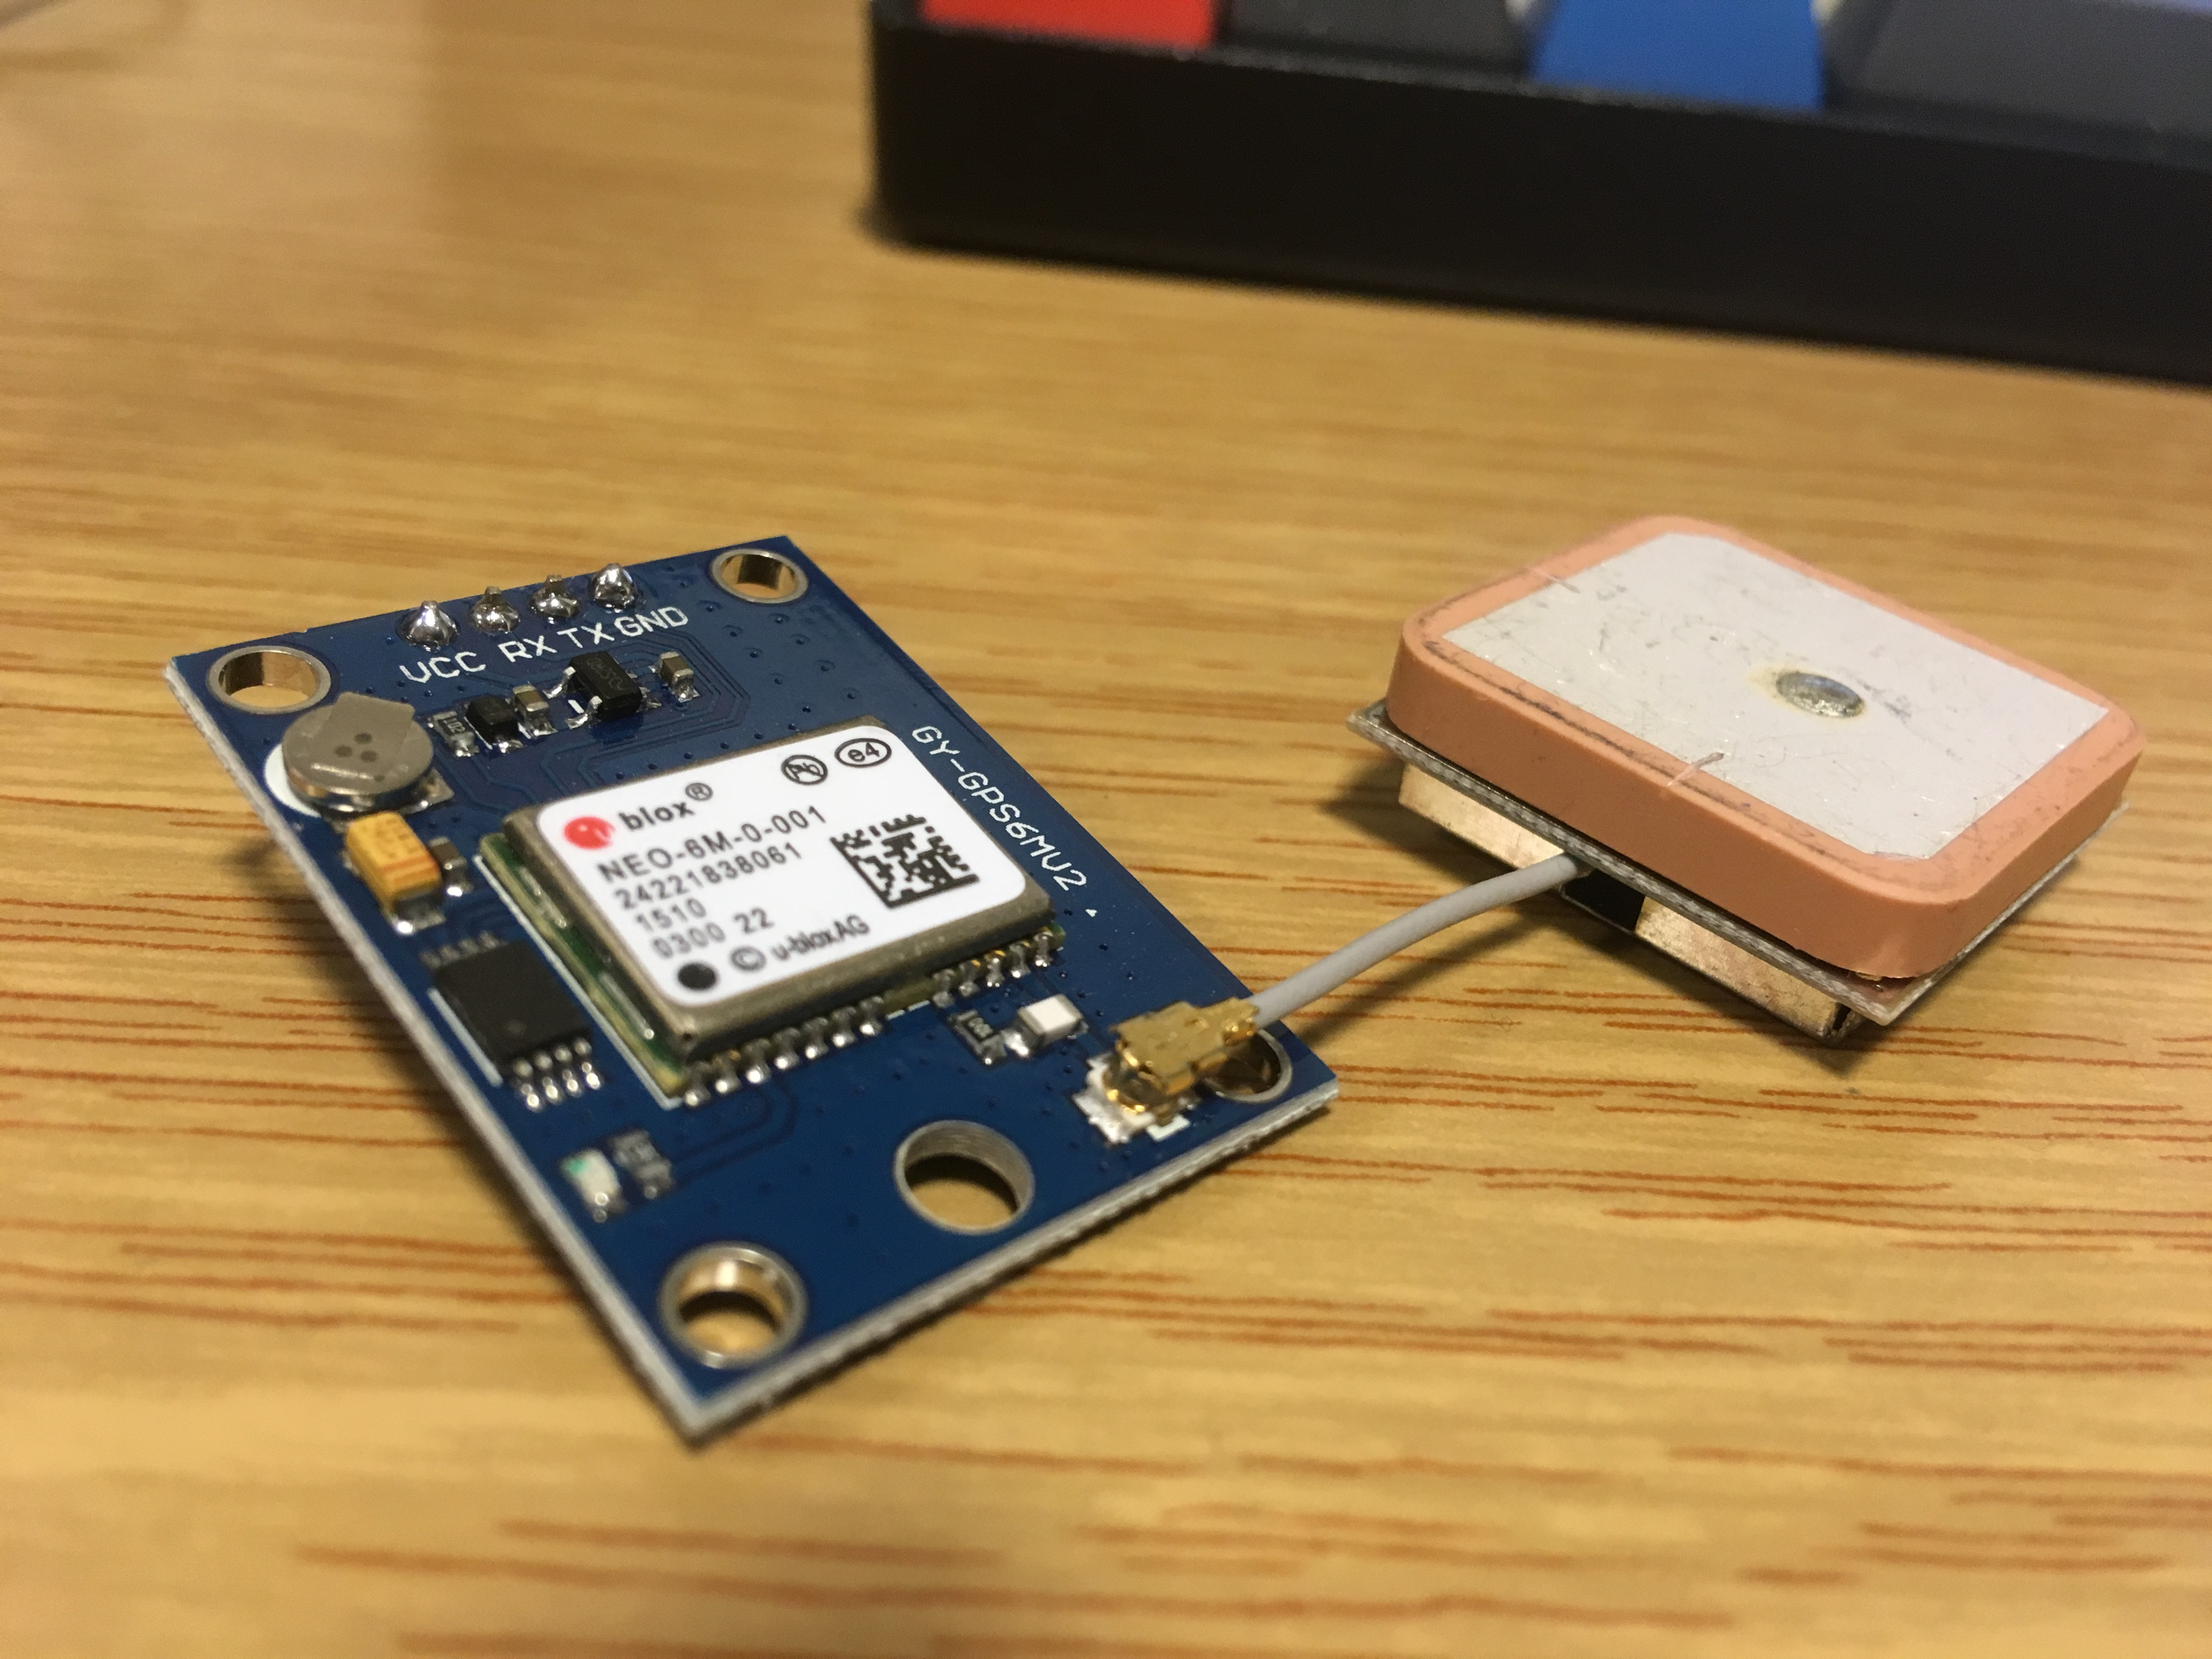
\includegraphics[width=0.7\linewidth]{gfx/walkerpictures/gps}
	\caption{Used GPS Module}
	\label{fig:walkerpictures_gps}
\end{figure}

\subsection{Heartrate Sensor}
The Heartrate Sensor iss a demonstration of what can be done [\ref{fig:walkerpictures_heartrate}].
\begin{figure}[h!]
	\centering
	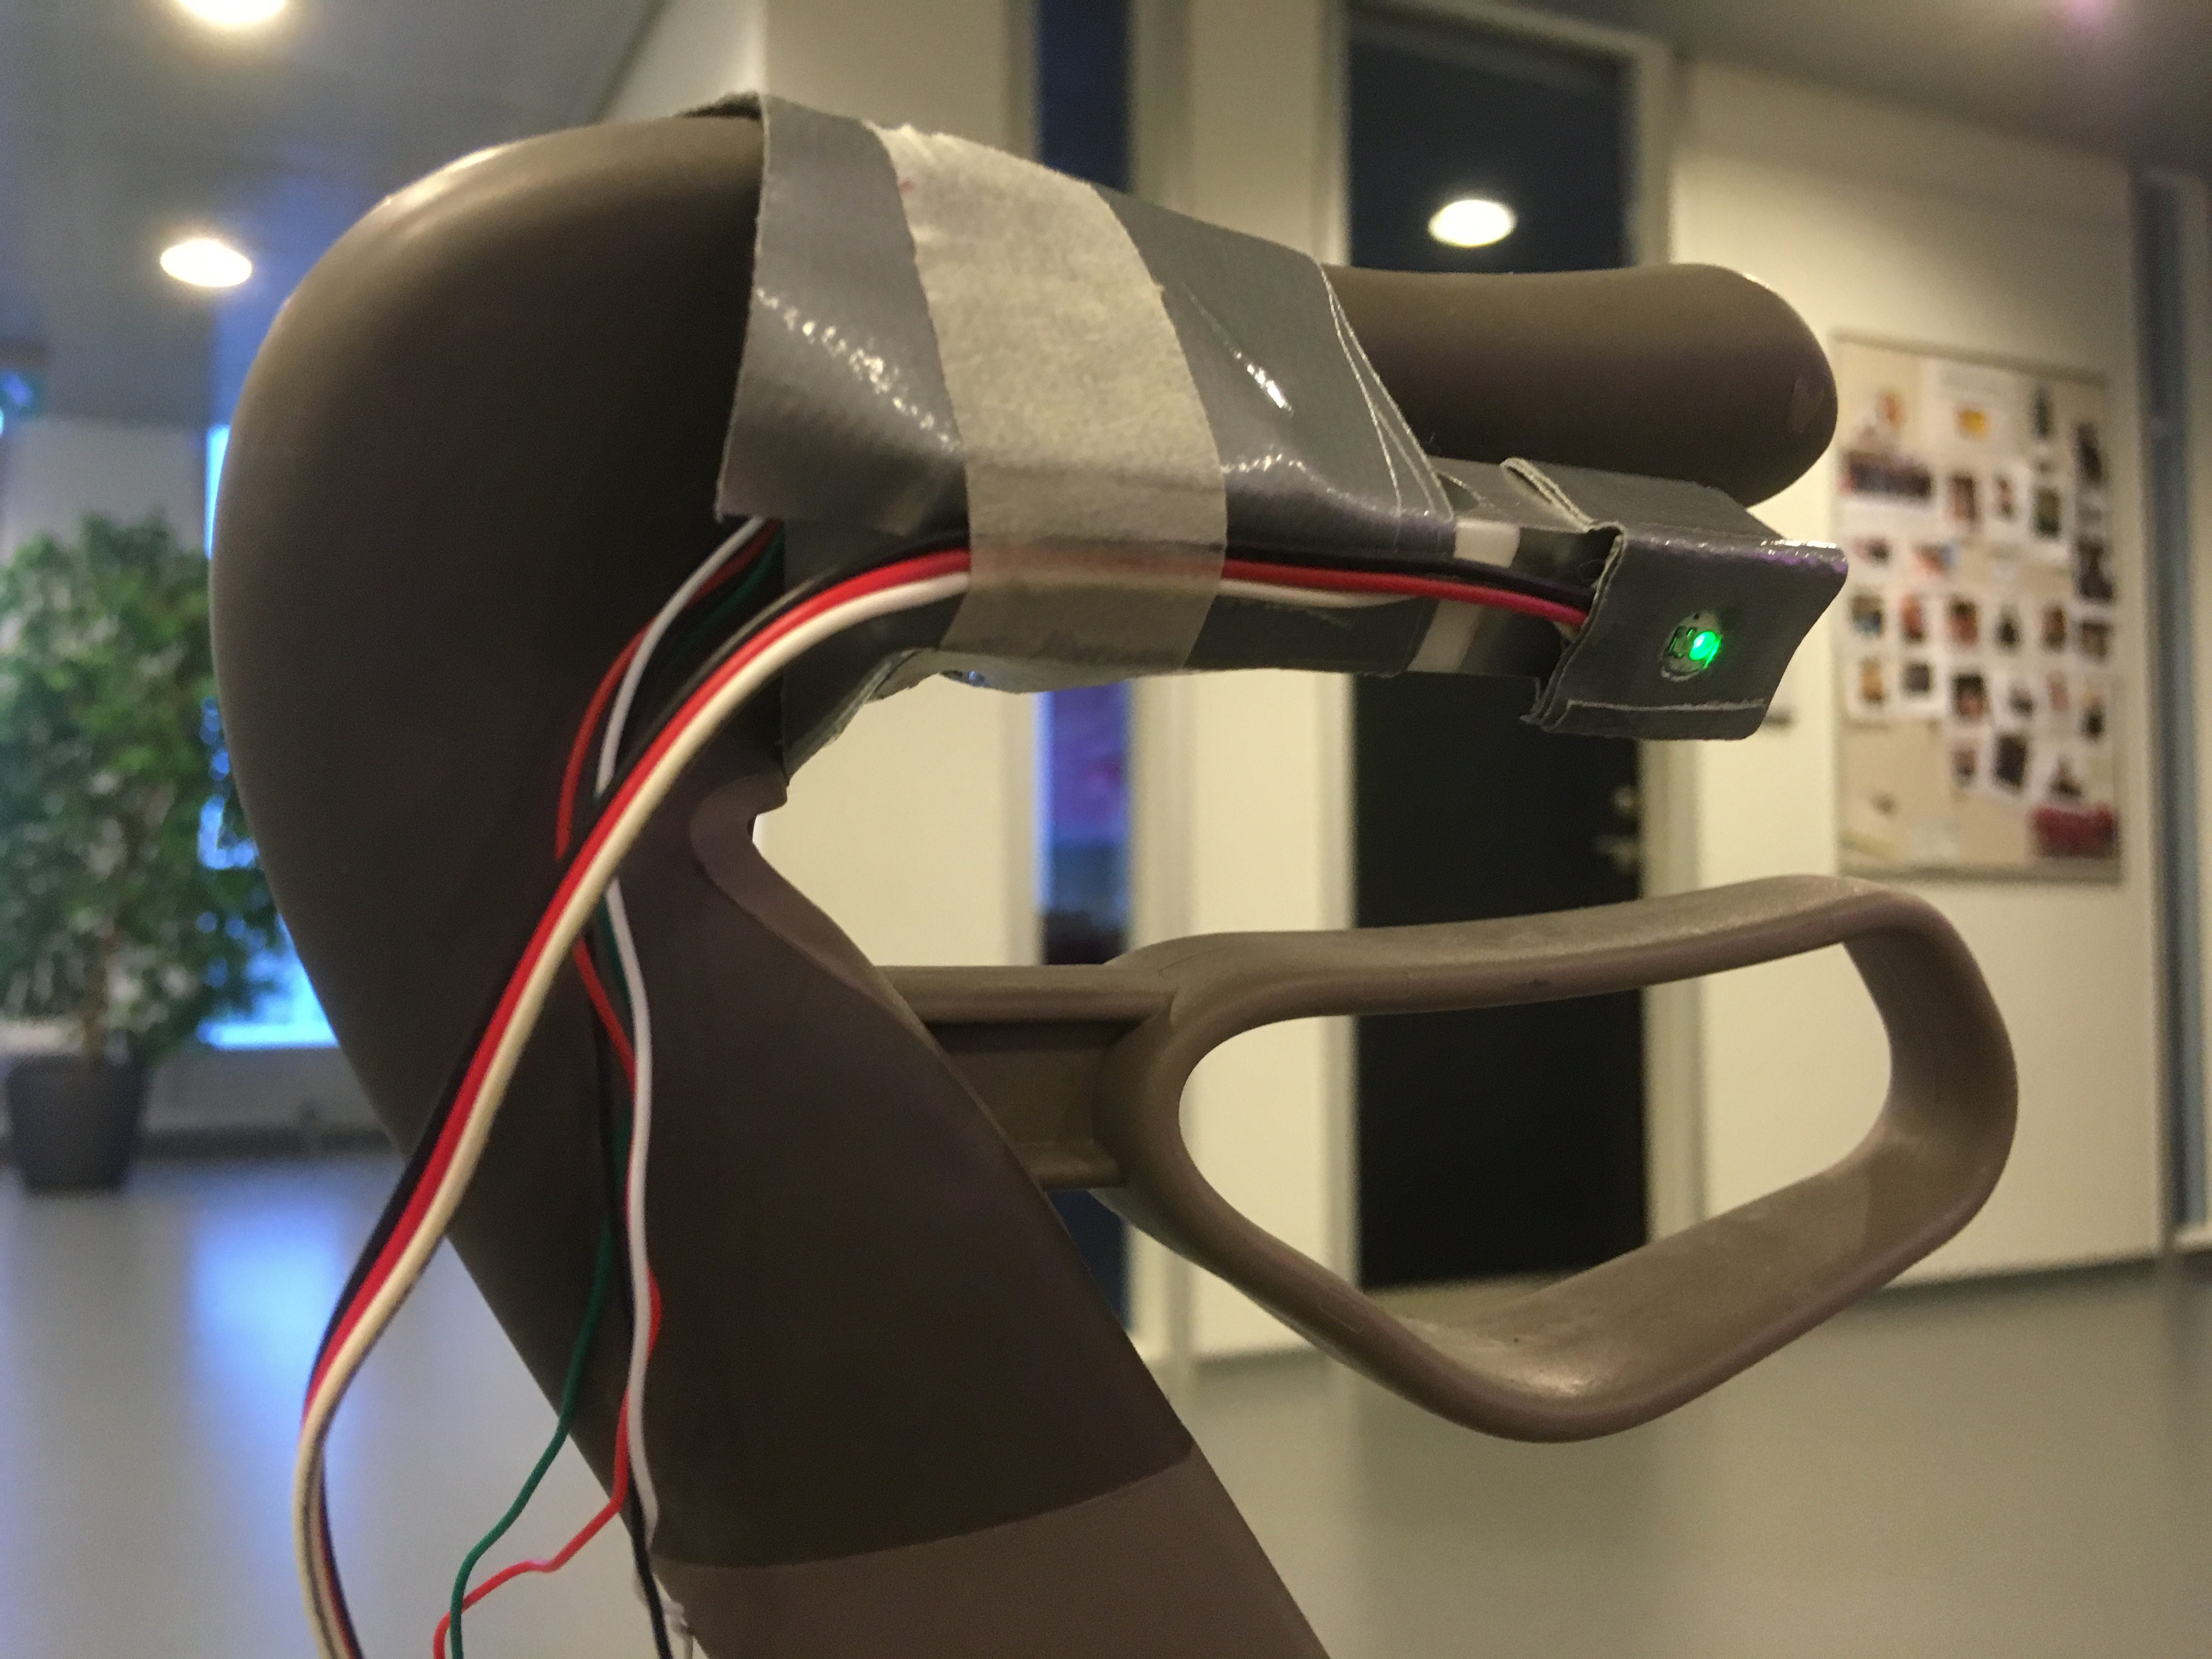
\includegraphics[width=0.7\linewidth]{gfx/walkerpictures/heartrate}
	\caption{Used Heartrate Sensor}
	\label{fig:walkerpictures_heartrate}
\end{figure}

\subsection{Movement Sensor}
The Movement Sensor allows us to measure the speed at which the user is walking. If we track both handles independently, together with the pressure measures, we can in a crude way analyse gait of the user [\ref{fig:walkerpictures_movement}].

\begin{figure}[h!]
	\centering
	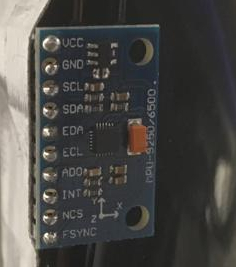
\includegraphics[width=0.7\linewidth]{gfx/walkerpictures/movement}
	\caption{Used Movement Sensor}
	\label{fig:walkerpictures_movement}
\end{figure}

\subsection{Pressure Sensors}
The Pressure Sensors allows to analyze how much the user relies on the walker over time and how the grip strength of the user changes over time [\ref{fig:walkerpictures_pressure}].
\begin{figure}[h!]
	\centering
	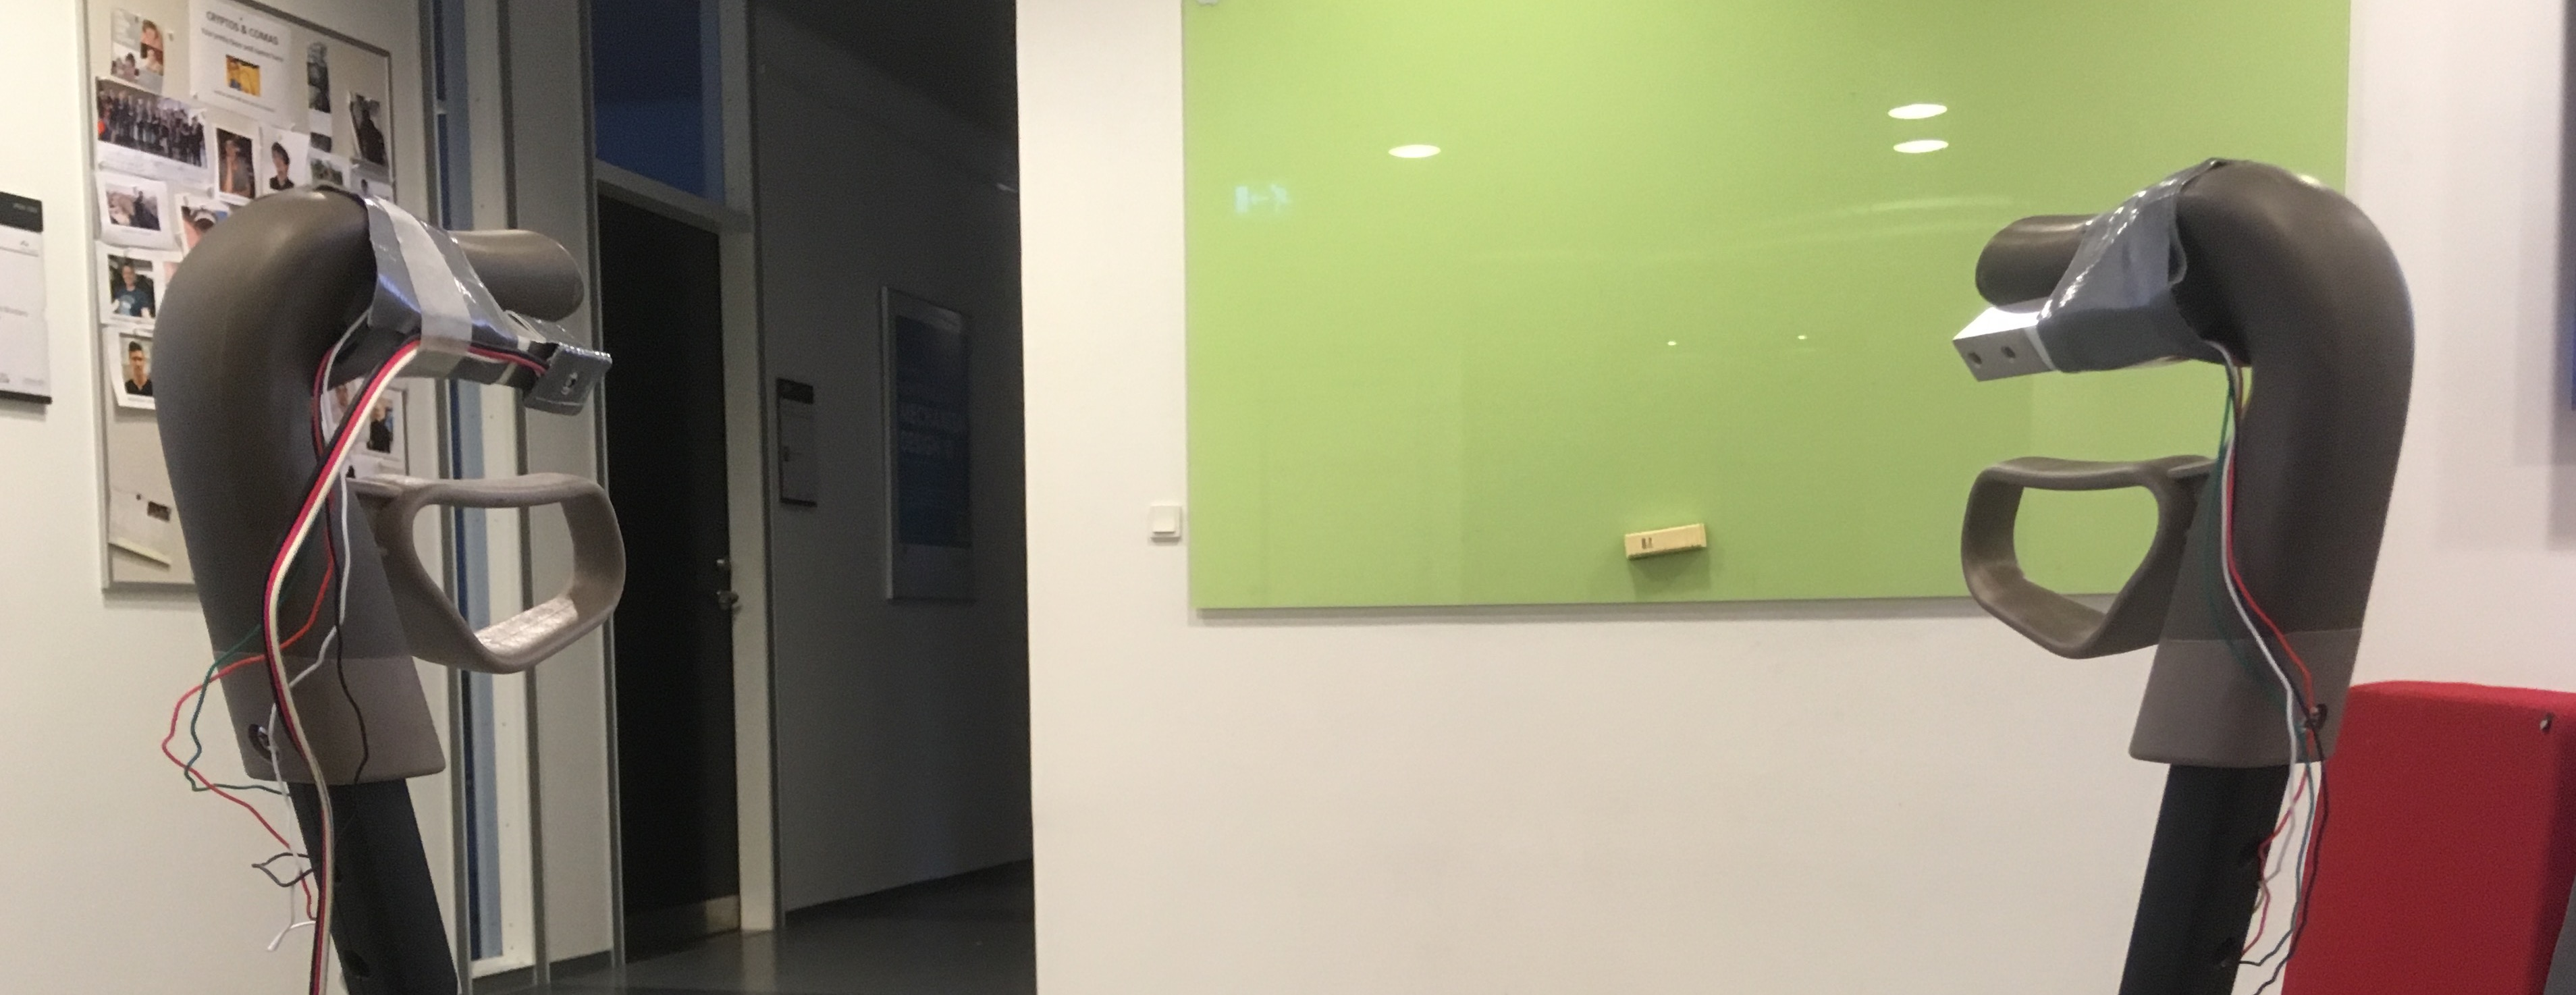
\includegraphics[width=0.7\linewidth]{gfx/walkerpictures/pressure}
	\caption{Used Pressure Sensors}
	\label{fig:walkerpictures_pressure}
\end{figure}


\subsection{LoRaWAN node}
A Arduino Mega with a LoRaWAN hat retreiving sensor data and connected to a battery [\ref{fig:walkerpictures_node}].
\begin{figure}[h!]
	\centering
	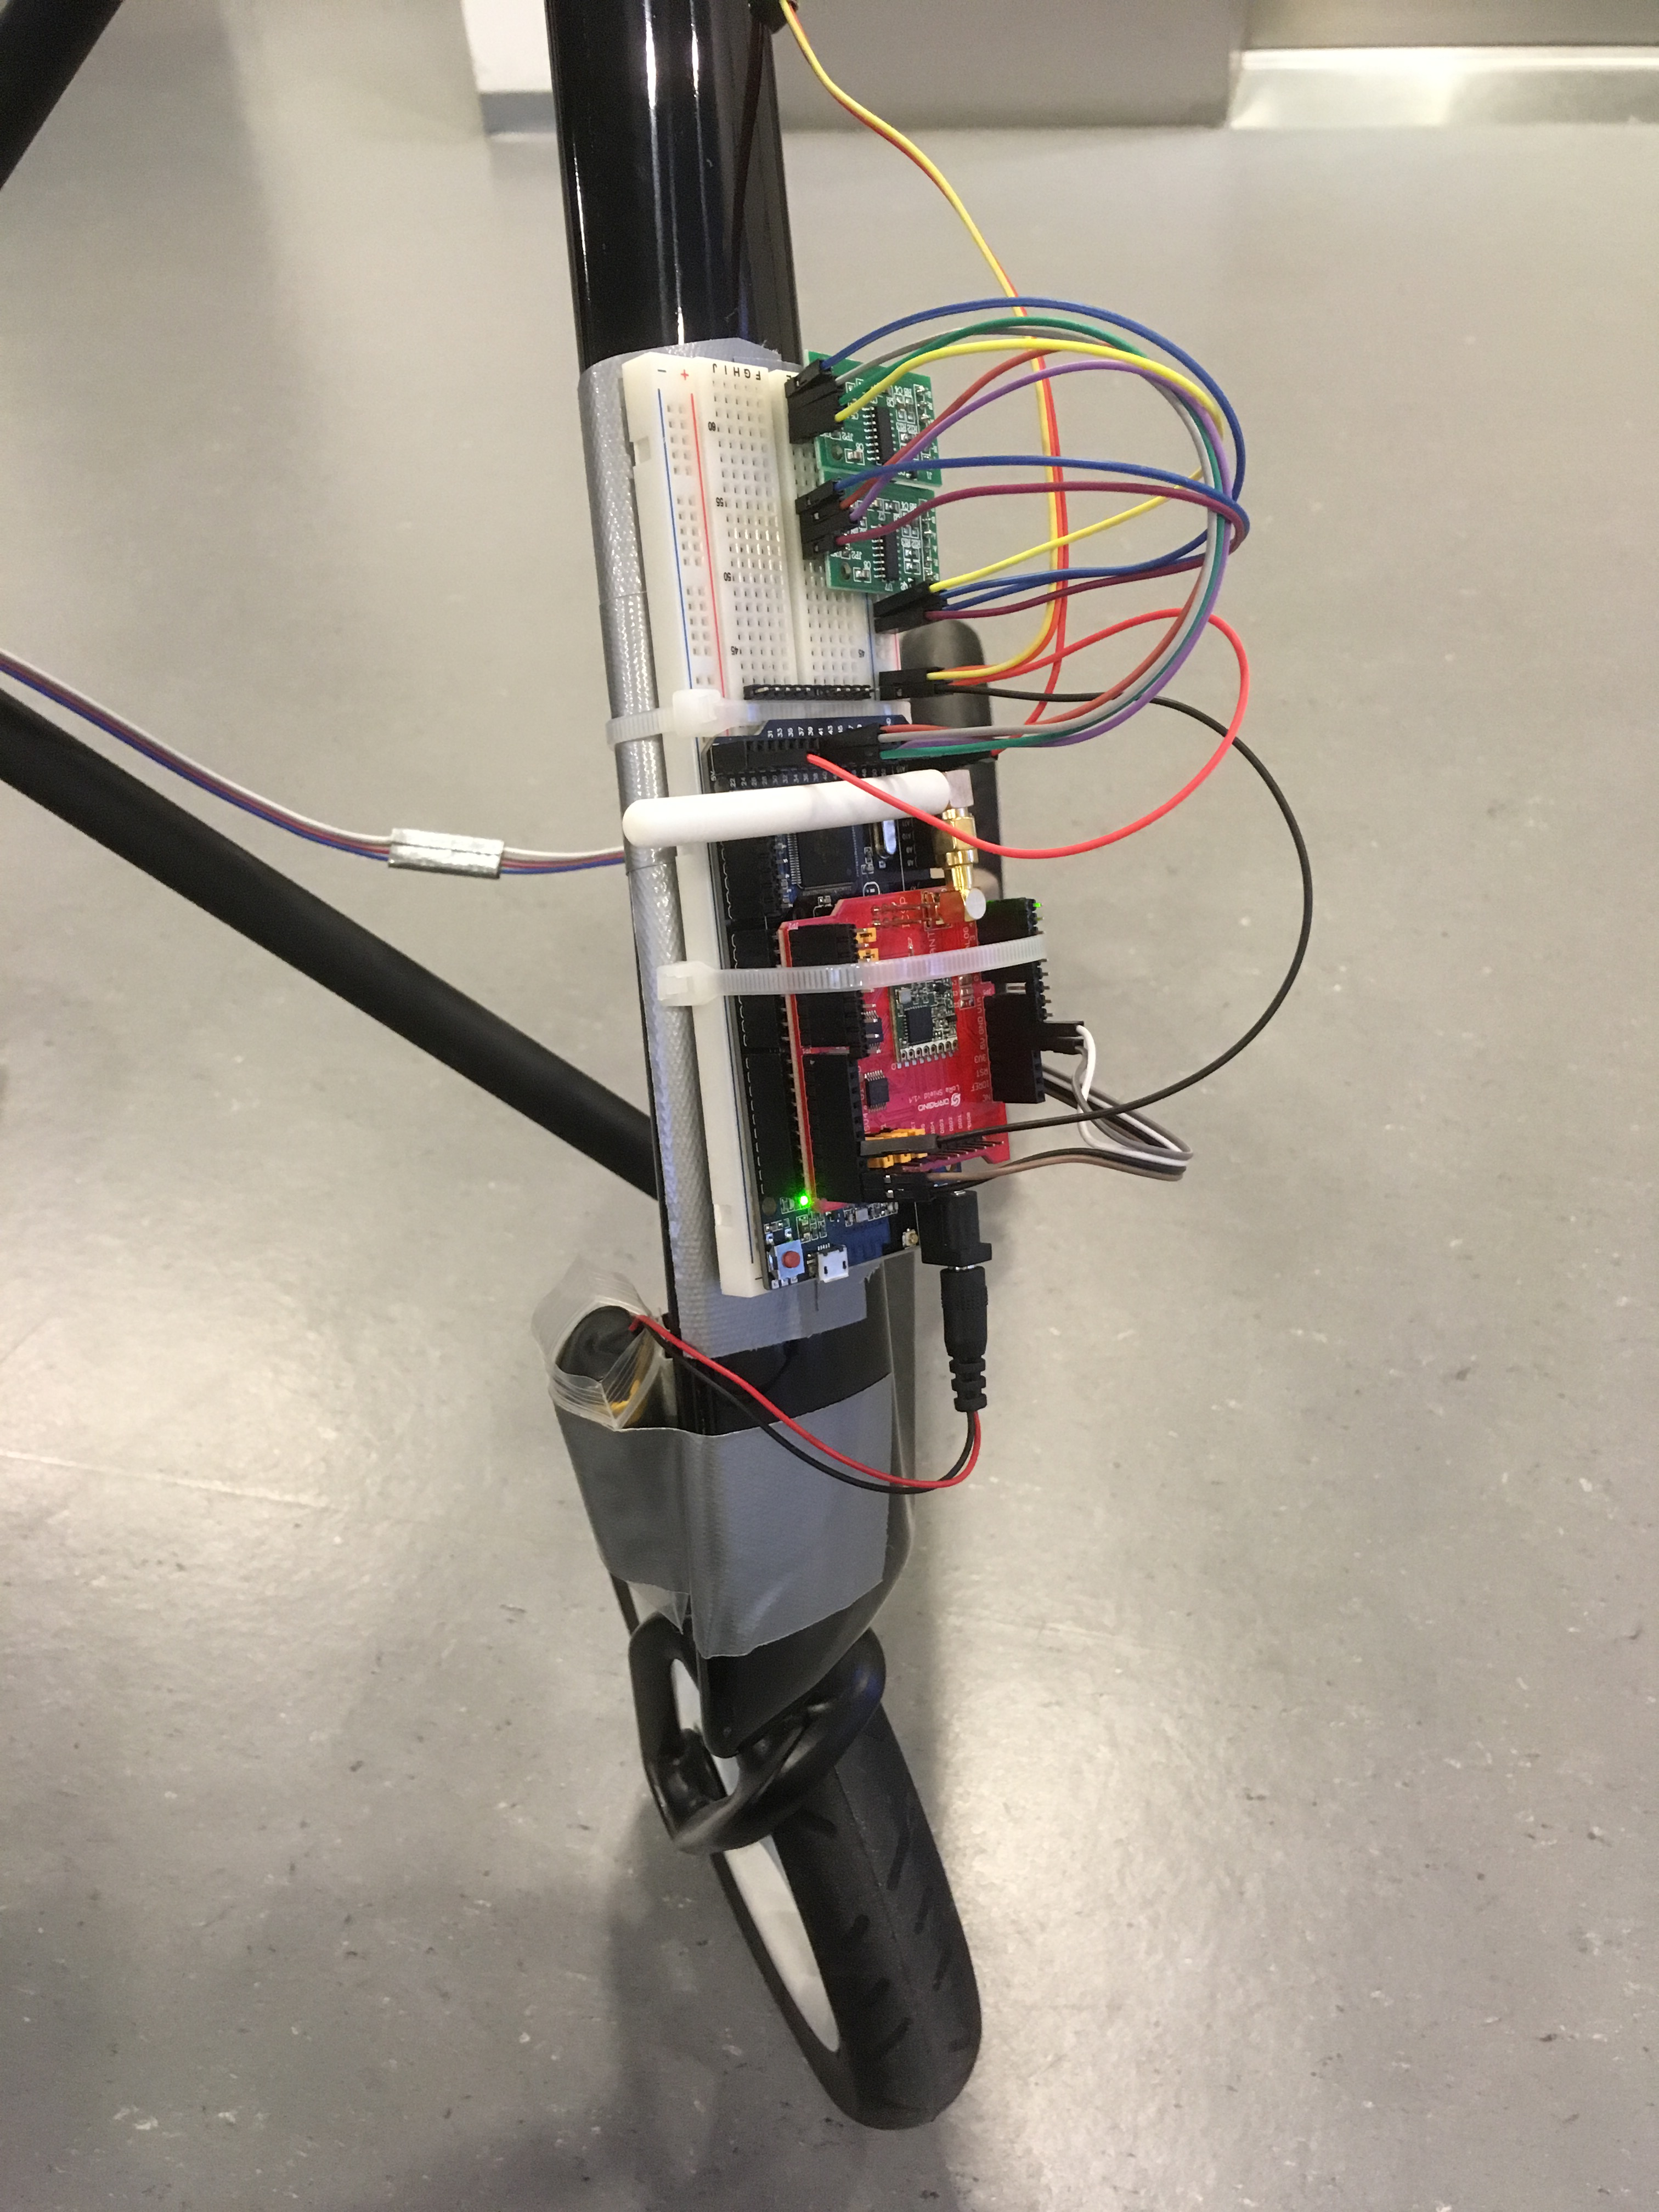
\includegraphics[width=0.7\linewidth]{gfx/walkerpictures/node}
	\caption{Used LoRaWAN node}
	\label{fig:walkerpictures_node}
\end{figure}
\newpage

\section{LoRaWAN gateway}
Raspberry Pi 3 with a LoRaWAN hat simply forwarding packets to The Things Network [\ref{fig:walkerpictures_gateway}].
\begin{figure}[h!]
	\centering
	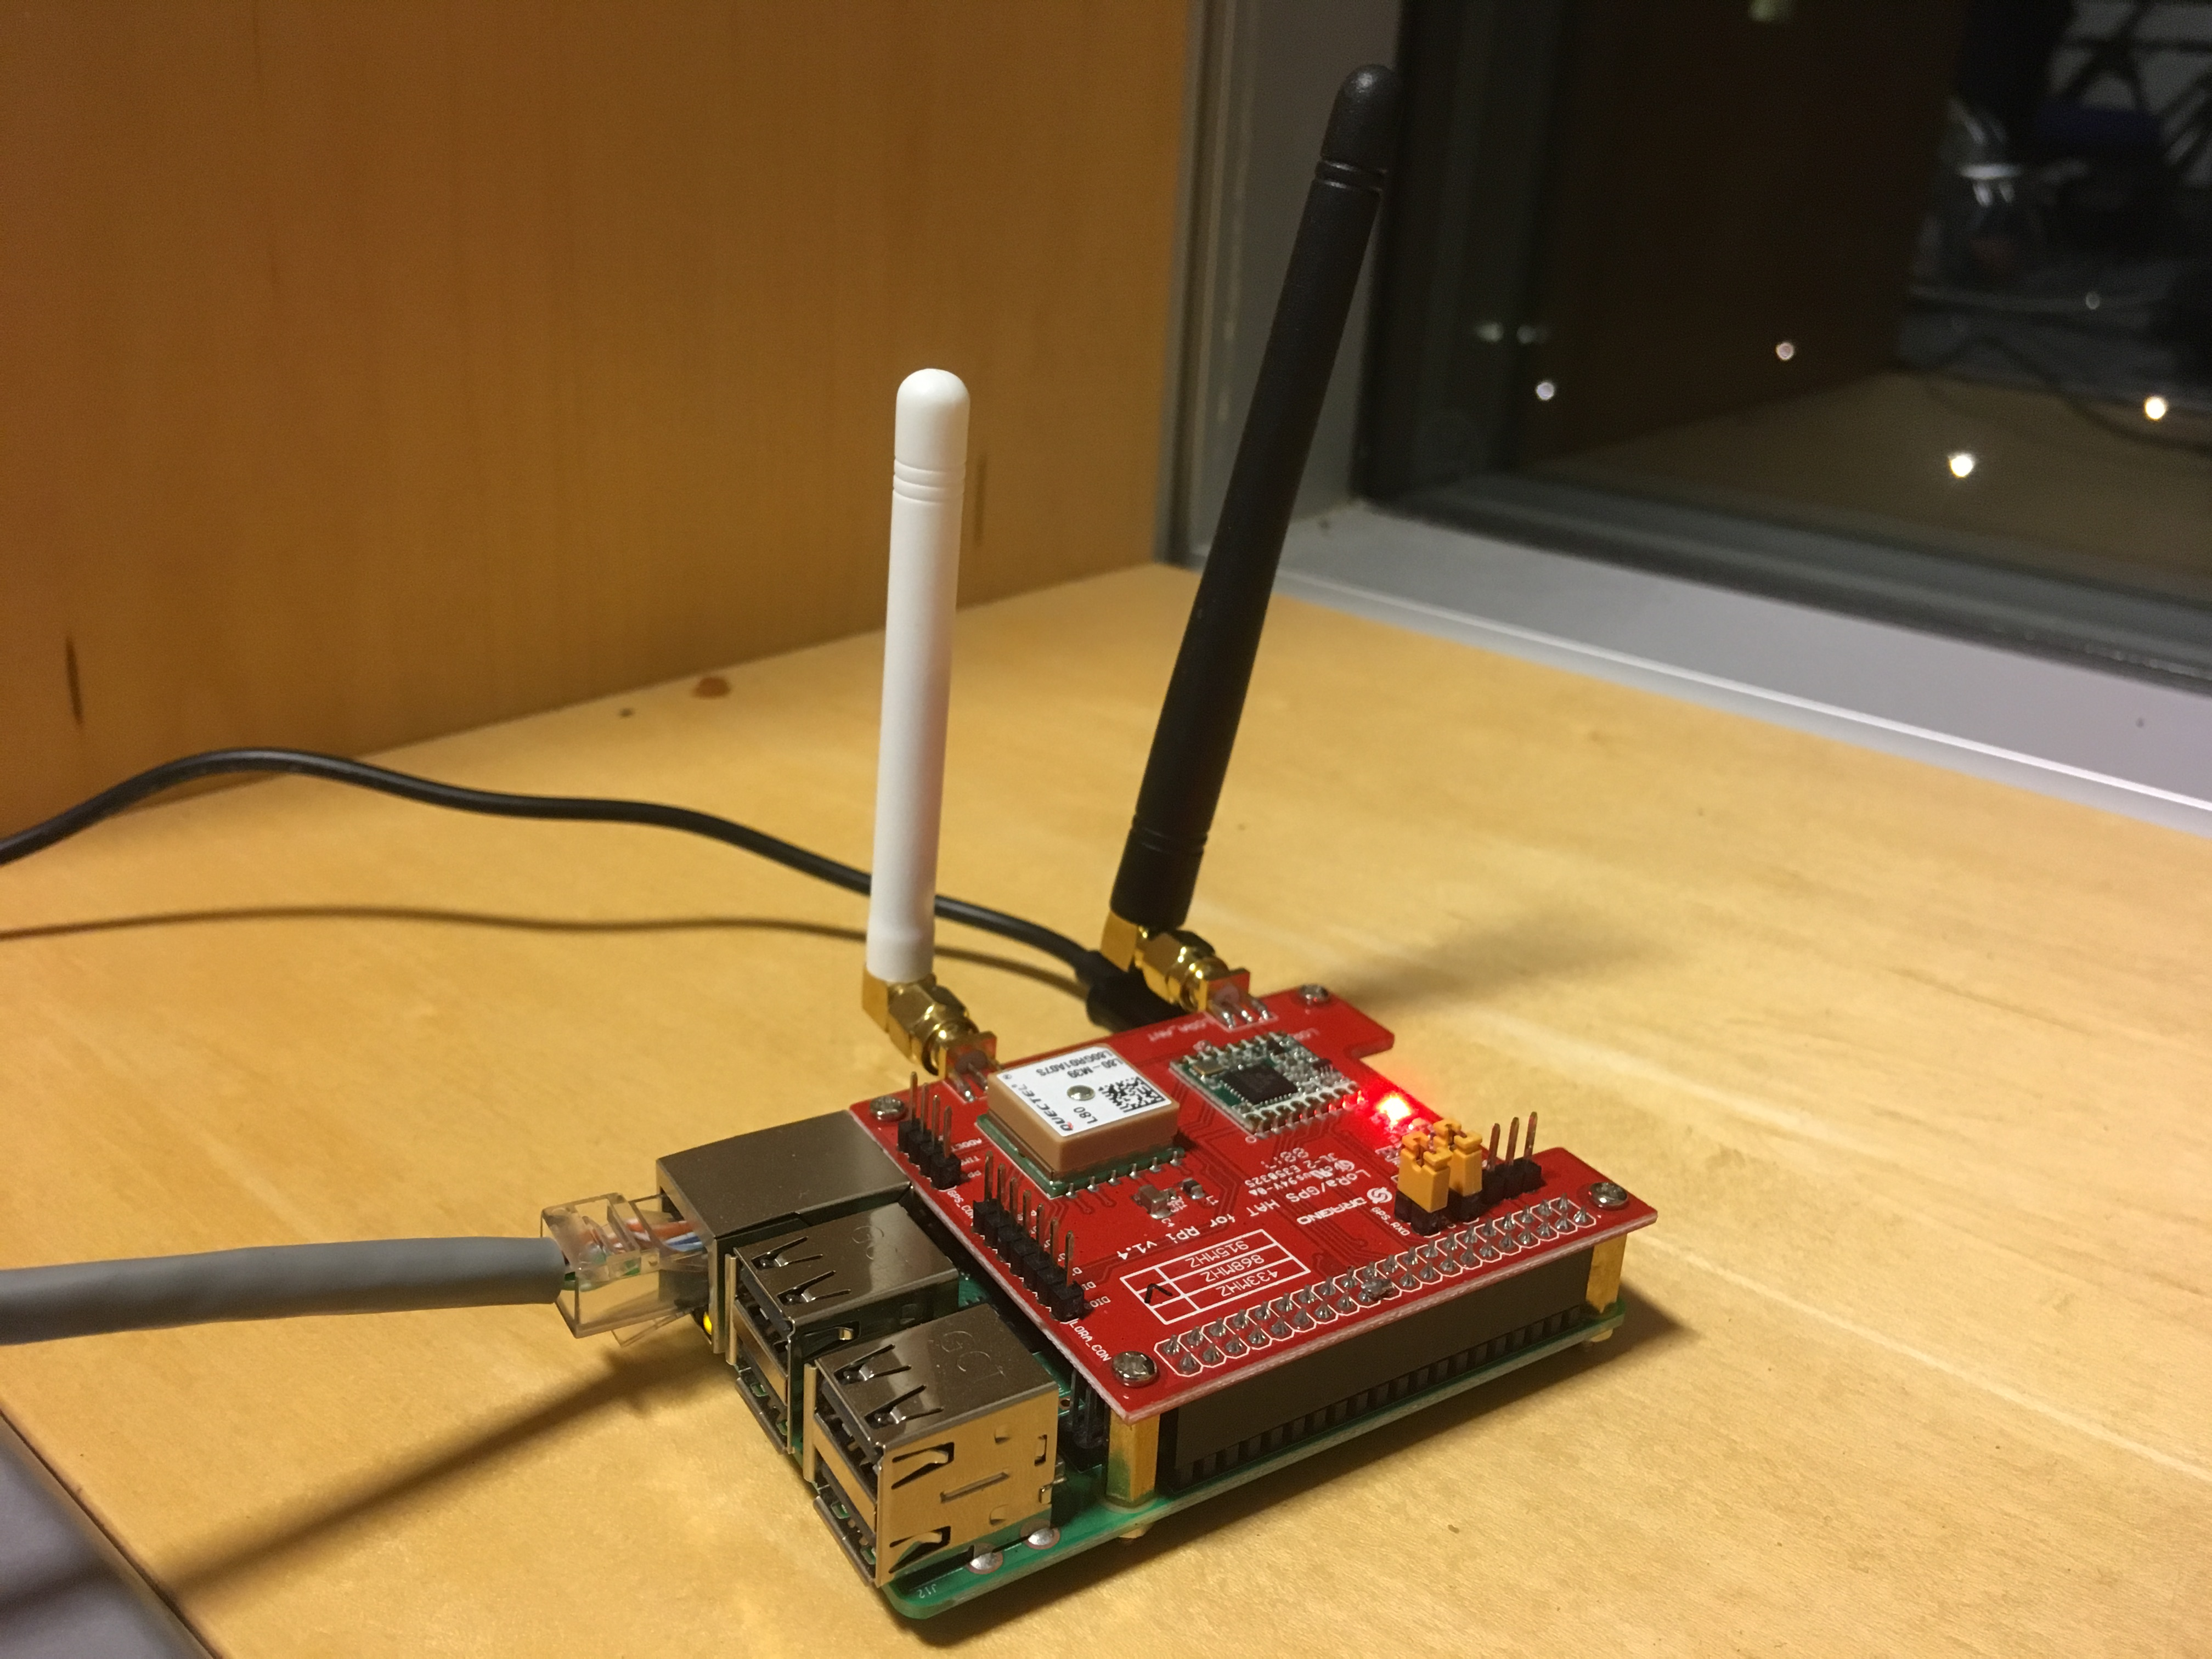
\includegraphics[width=0.7\linewidth]{gfx/walkerpictures/gateway}
	\caption{Used LoRaWAN gateway}
	\label{fig:walkerpictures_gateway}
\end{figure}

\section{Product Video}
In the following you can find a demonstration of the project:\\
https://vimeo.com/304645369

